\documentclass[11pt]{article}
%Gummi|061|=)
\usepackage[italian]{babel}
\usepackage[utf8x]{inputenc}
\usepackage{hyperref}
\usepackage{graphicx}
\usepackage{amsmath}
\DeclareMathOperator{\Tr}{Tr}
\DeclareMathOperator{\Exp}{exp}
\DeclareMathOperator{\Log}{log}
\DeclareMathOperator{\Det}{det}

\title{}
\author{}
\date{}
\begin{document}

\maketitle


\section{Vdovichenko 1}
\noindent
Nel capitolo precedente avevamo considerato due diverse costanti di accoppiamento $J$ e $J'$ con il solo scopo di separare le variabili $v$ e $w$, il ché ci ha permesso di comprendere meglio la configurazione grafica dei termini $v^rw^s$ sul reticolo.\\
D'ora in poi per semplicità considereremo $J=J'$ e quindi $v=w$: stiamo dicendo che i termini $v^4w^2$ e $v^2w^4$ della \ref{primiserie} ora compaiono tutti come $v^6$ con degenerazione $2N$. \\
Definiamo inoltre come \emph{maglia} una sola poligonale chiusa, come \emph{grafico} l'unione di una o più maglie.  \\
La funzione di partizione diventa dunque
\begin{equation}\label{enlib}
Z_N=2^N(1-v^2)^{-N}\Phi(v)
\end{equation}
con 
\begin{equation}
\Phi(v)= \sum_r g_r v^r
\end{equation}
dove $g_r$ è il numero di grafici non necessariamente connessi con perimetro $r$ accendibili sul reticolo. \\
L'obbiettivo di questo capitolo è scrivere i grafici che avevamo acceso sul reticolo nello sviluppo ad alte temperature come dei \emph{cammini chiusi}. \\
Il problema sorge davanti a grafici ambigui come quello in figura \ref{v1}, che può essere interpretato nei tre modi descritti.
\begin{figure}[h]
\centering
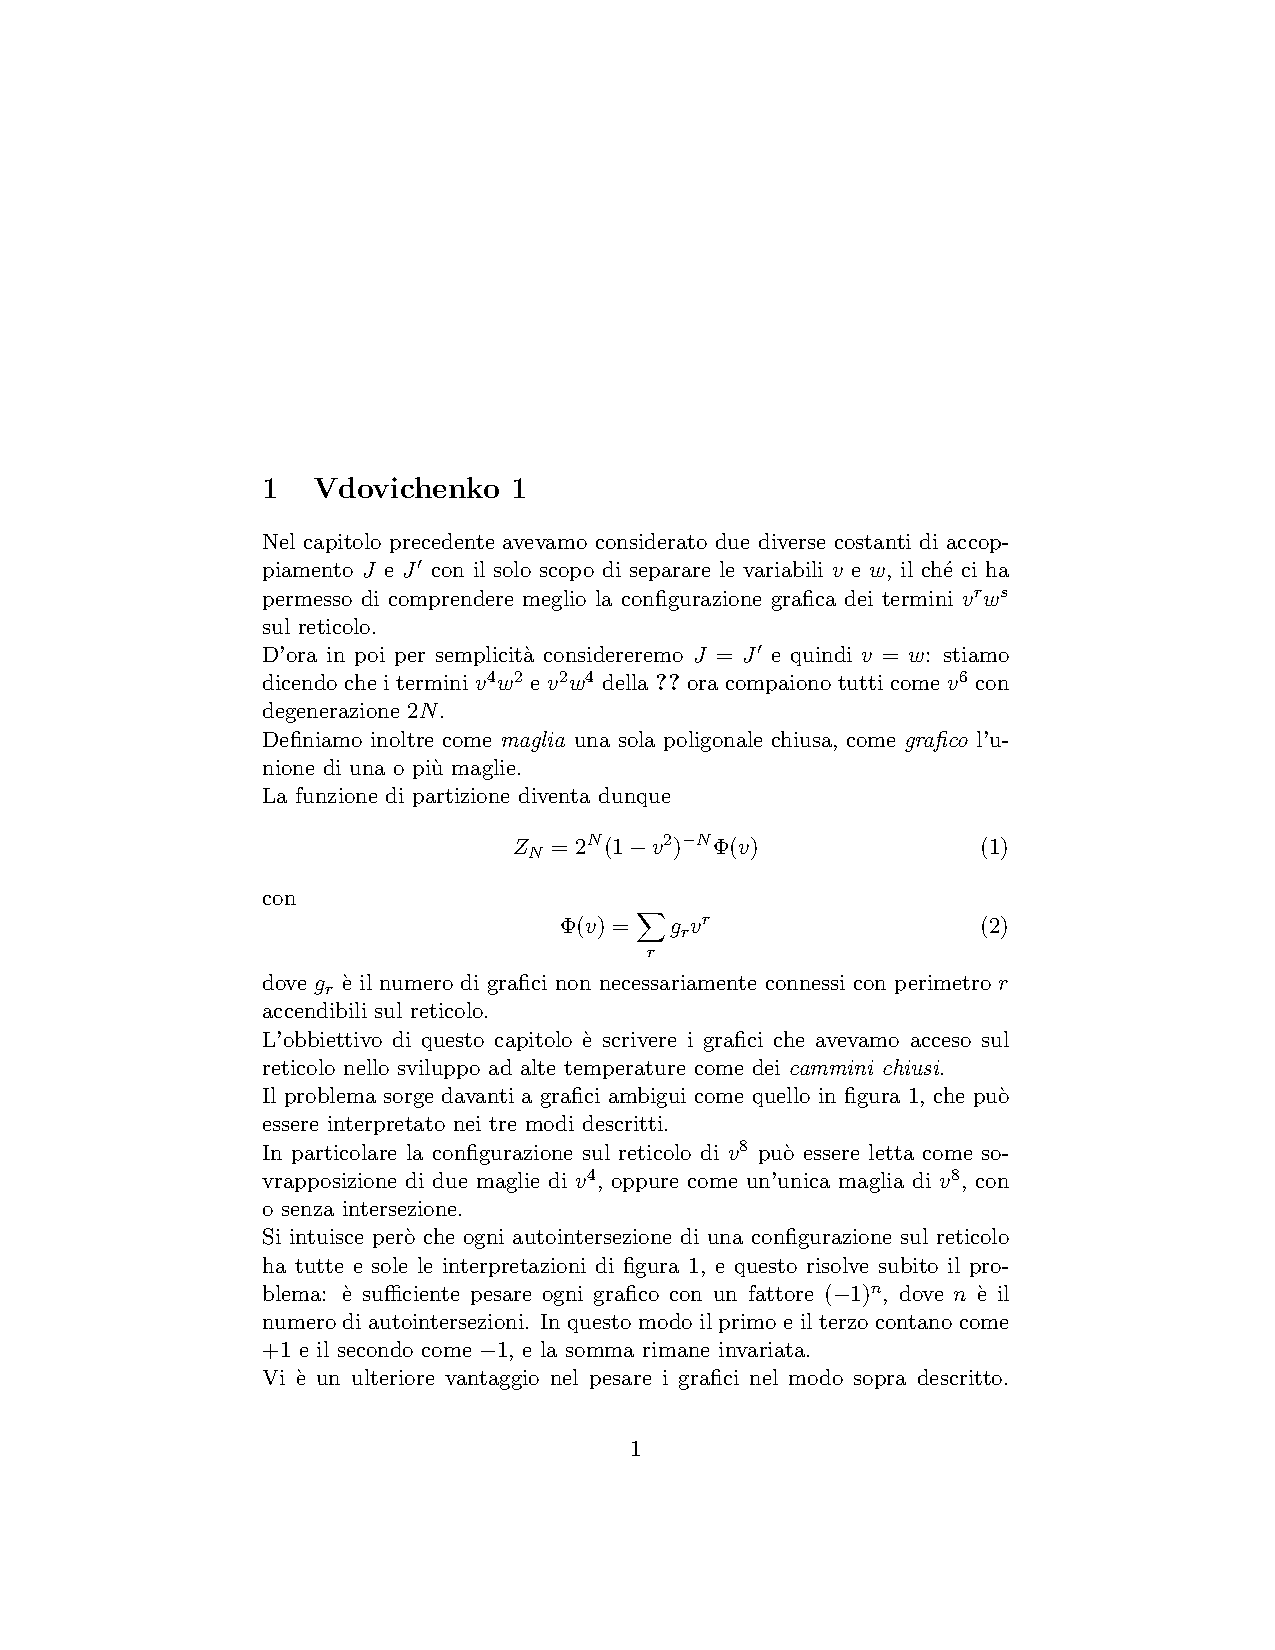
\includegraphics[width=0.5\columnwidth]{v1}
\caption{tre diversi grafici di $v^8$ con identica configurazione sul reticolo}
\label{v1}
\end{figure}
\\
In particolare la configurazione sul reticolo di $v^8$ può essere letta come sovrapposizione di due maglie di $v^4$, oppure come un'unica maglia di $v^8$, con o senza intersezione.\\
Si intuisce però che ogni autointersezione di una configurazione sul reticolo ha tutte e sole le interpretazioni di figura \ref{v1}, e questo risolve subito il problema: è sufficiente pesare ogni grafico con un fattore $(-1)^n$, dove $n$ è il numero di autointersezioni. In questo modo il primo e il terzo contano come $+1$ e il secondo come $-1$, e la somma rimane invariata.\\
Vi è un ulteriore vantaggio nel pesare i grafici nel modo sopra descritto. Come accennato precedentemente non è ammissibile come configurazione grafica sul reticolo di $v^8$ quella formata da due quadrati con un lato in comune: i due siti centrali avrebbero un numero dispari di ingressi/uscite, $\sigma_i$ sarebbe elevata al cubo, ed essendo antisimmetrica verrebbe, come già spiegato, eliminato. Nel caso però venissero contati, se pesati con il fattore $(-1)^n$ non darebbero comunque contributo, in quanto si eliminerebbero a vicenda. Si veda la figura \ref{v2} per capire come.
\begin{figure}[h]
\centering
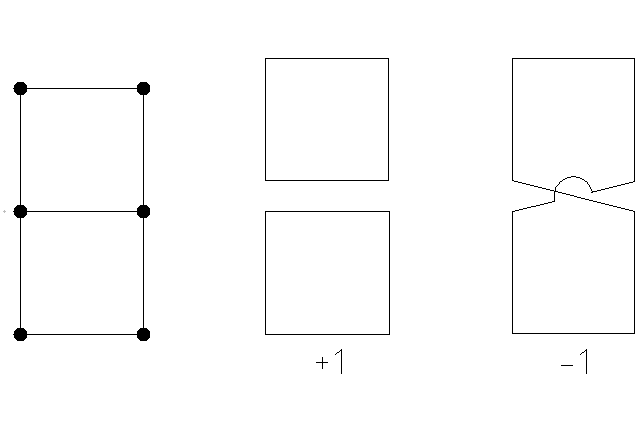
\includegraphics[width=0.4\columnwidth]{v2}
\caption{tre diversi grafici di $v^8$ con identica configurazione sul reticolo}
\label{v2}
\end{figure}
\\
Bisogna quindi capire come determinare il numero di autointersezioni $n$ di una maglia. Il problema risiede nel fatto che questa è una proprietà globale, mentre noi lavoriamo in maniera locale, ovvero guardando spigolo dopo spigolo cosa succede. \\
Il metodo che si utilizza è discendente del noto teorema di Gauss che afferma che l'angolo spazzato dalla tangente su un cammino chiuso senza intersezioni è $2\pi$. Generalizzando si intuisce che questo angolo è $2\pi(k+1)$, con $k$ intero postivo o negativo che aumenta o diminuisce a seconda che le intersezioni avvengano in un verso oppure nell'altro, come spiegato intuitivamente in figura \ref{v3}.
\begin{figure}[h]
\centering
\includegraphics[width=0.8\columnwidth]{v3}
\caption{Generalizzazione del teorema di Gauss sull'angolo spazzato dalla tangente di una curva}
\label{v3}
\end{figure}
\\ La procedura da seguire è la seguente: ad ogni punto del cammino corrisponde un angolo di rotazione che può essere $\alpha=0;\pm\pi/2$, gli si associa una fase $e^{i\alpha/2}$ e si ottiene, dopo aver camminato su tutta la maglia, il valore $(-1)^{\nu+1}$, con $\nu$ somma delle intersezioni di una maglia, pesate del loro segno. Per un insieme di più maglie si ottiene $(-1)^{n+s}$ con $n=\sum\nu$ e $s$ numero di maglie. Ovviamente noi vorremmo ad esponente solo $n$ e non $s$, dopo vedremo come risolvere questo inconveniente.\\
Chiamiamo ora con $f_r$ il numero di maglie di perimetro $r$ pesate nel modo sopra descritto. Il numero dei grafici composti da due maglie pesate sarà
$$\frac{1}{2!}\sum_{r_1+r_2=r}f_{r_1}f_{r_2}$$
dove ovviamente il $2!$ è necessario in quanto i grafici sono indistinguibili. Qui torna molto utile quanto discusso nella \ref{v2}, in quanto avremmo dovuto altrimenti fare un calcolo più complesso. Un generico grafico è composto da $s$ maglie, con $s$ variabile da $1$ a $+\infty$, quindi si scrive
\begin{equation} \label{phi}
\Phi(v)=\sum_{s=0}(-1)^s\frac{1}{s!}\sum_{r_1,r_2,...=1}^\infty v^{r_1+r_2+...r_s}f_{r_1}...f_{r_s}
\end{equation}
Il fattore $(-1)^s$ serve a compensare il seguente inconveniente lasciato in sospeso poche righe sopra, $\frac{1}{s!}$ è l'estensione dell'$\frac{1}{2!}$. Notiamo che gli esponenti $r_i$ assumono tutti i possibili valori da $1$ a $+\infty$ in tutte le possibili combinazioni, quindi anche $r=\sum_i r_i$. Possiamo quindi riorganizzare la sommatoria come
$$\sum_{r_1,r_2...=1}^\infty v^{r_1+r_2+...r_s}f_{r_1}...f_{r_s}=\left( \sum_{r=1}^\infty v^rf_r \right)^s$$
e sostituirla nell'equazione \ref{phi}, che riconosciamo subito essere uno sviluppo in serie di un esponenziale:
\begin{equation}\label{phi2}
 \Phi(v)= \exp \left[ - \sum_{r=1}^\infty v^r f_r \right]
\end{equation}
Resta da determinare la quantità $f_r$.\\
Iniziamo indicizzando con $\mu=1,2,3,4$ gli spostamenti sul reticolo rispettivamente verso destra, in alto, sinistra, in basso.
L'informazione che daremo d'ora in avanti sarà sempre nella forma
$$ (coordinate \ del \ sito, \ direzione \ di \ ingresso \ nel \ sito)
$$
Decidiamo quindi di partire dal sito di coordinate $(i_0,j_0)$ con direzione \emph{di ingresso} in detto sito $\mu_0$. Notiamo che questa direzione non ha alcuna influenza sul cammino che stiamo per descrivere. Possiamo così introdurre la funzione $W_r(i,j,\mu)$ come il numero pesato di cammini che arrivano al punto $(i,j)$ con direzione $\mu$ dopo $r$ passi data o meno una condizione iniziale. Poniamo inoltre per comodità $\mu=\mu_0$, tanto come già detto $\mu_0$ non ha influenza sul cammino che stiamo per percorrere. Alcuni esempi dati $(i_0,j_0,\mu_0)=(0,0,1)$ sono (si veda la figura \ref{v6}):
\begin{itemize}
\item{$W_1(1,0,1)=1$ dobbiamo partire da $(0,0)$ diretti verso destra e dobbiamo arrivare in $(1,0)$ da sinistra. Ovviamente c'è solo una possibilità}
\item{$W_2(1,1,4)=e^{i\frac{\pi}{4}}$ anche qui una sola possibilità}
\item{$W_4(0,0,4)=2$}
\item{$W_8(0,0,4)=1+1+1+1=4$ decisamente meno intuitiva}
\end{itemize}
\begin{figure}[h]
\centering
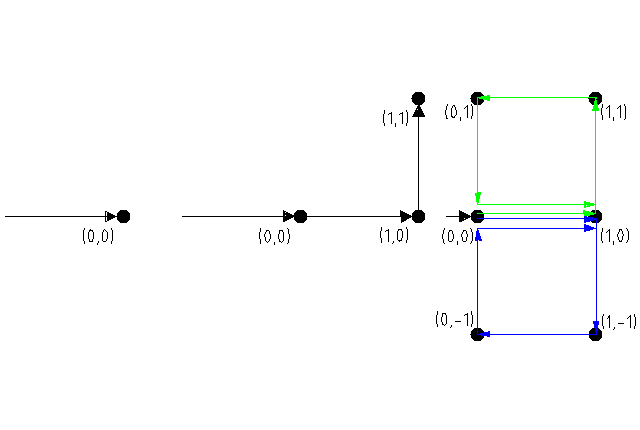
\includegraphics[width=0.8\columnwidth]{v6}
\caption{esempi di camini sul reticolo}
\label{v6}
\end{figure}
 Questo siglifica che se scriviamo $W_r(i_0,j_0,\mu)$ sto chiedento il numero pesato di cammini che partono in $(i_0,j_0)$ dopo esserci arrivati con direzione $\mu_0=\mu$, e ci ritornano dopo $r$ passi nella direzione $\mu$. Possiamo quindi scrivere
 $$ f_r=\frac{1}{2r}\sum_{i_0,j_0,\mu}W_r(i_0,j_0,\mu)
 $$
dove l'$\frac{1}{2r}$ è necessario in quanto nella sommatoria un solo cammino è percorso nei due versi e partendo da ognuno dei suoi $r$ punti. 
La funzione $W_r(i,j,\mu)$ gode di proprietà ricorsive ben definite e facilmente intuibili, nella figura \ref{v7} rappresentiamo graficamente la prima.
$$
\begin{array}{lcl} 
W_{r+1}(i,j,1) & = & W_r(i-1,j,1)+e^{-i\frac{\pi}{4}}W_r(i-1,j,2)+0+e^{i\frac{\pi}{4}}W_r(i-1,j,4) \\
W_{r+1}(i,j,2) & = & e^{i\frac{\pi}{4}}W_r(i,j-1,1)+W_r(i,j-1,2)+e^{-i\frac{\pi}{4}}W_r(i,j-1,3)+0 \\
W_{r+1}(i,j,3) & = & 0+e^{i\frac{\pi}{4}}W_r(i+1,j,2)+W_r(i+1,j,3)+e^{-i\frac{\pi}{4}}W_r(i+1,j,4) \\
W_{r+1}(i,j,4) & = & e^{-i\frac{\pi}{4}}W_r(i,j+1,2)+0+e^{i\frac{\pi}{4}}W_r(i,j+1,3)+W_r(i,j+1,4)
\end{array} 
$$
\begin{figure}[h]
\centering
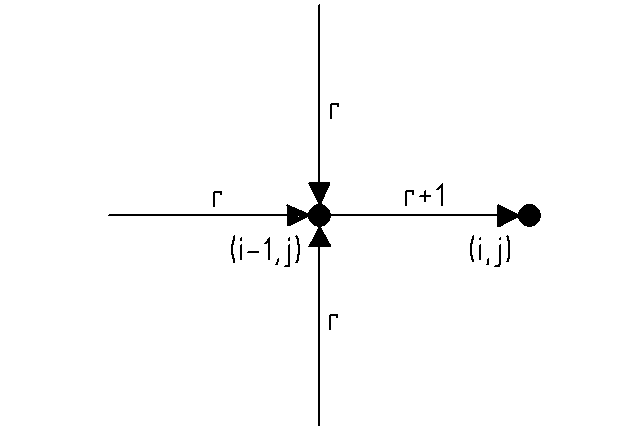
\includegraphics[width=0.8\columnwidth]{v7}
\caption{esempi di camini sul reticolo}
\label{v7}
\end{figure}
Come per ogni funzione ricorsiva, ad un certo punto arriviamo a chiederci quanto valga $W_1$. Questa funzione è perfettamente determinata dalle condizioni iniziali. \\
Esiste quindi un'applicazione lineare con matrice associata $\Lambda$ tale per cui
\begin{equation}
W_{r+1}(i,j,\mu)=\sum_{i',j',\mu',\mu_0}\Lambda(ij\mu|i'j'\mu')W_{r}(i',j',\mu')
\end{equation}
Notiamo che $\Lambda$ è funzione non solo degli indici direzionali $\mu$ e $\mu'$, che variano da 1 a 4, ma anche di quelli di posizione. Stiamo quindi parlando di una matrice di grosse dimensioni.\\
Notiamo subito l'analogia tra il comportamento della matrice $\Lambda$ e quello degli operatori nella Meccanica Quantistica: in entrambi i casi sono oggetti che descrivono la transizione del sistema da uno stato all'altro. Nel nostro caso particolare, dato un certo sito del reticolo, $\Lambda$ mi serve a capire quali sono gli spostamenti permessi. Il modulo quadro dei suoi coefficienti $\Lambda_{ij \mu | i'j' \mu'}$, sempre in analogia con la Meccanica Quantistica, rappresentano la probabilità di transizione da un sito all'altro.\\
Con quest'ultima interpretazione della matrice $\Lambda$, è chiaro cosa rappresentano i generici $\langle i,j,\mu|_r |i_0,j_0,\mu_0\rangle_0$: sono il numero di modi (quindi la probabilità) di partire dal sito $(i_0,j_0)$ dopo esserci arrivati con direzione $\mu_0$ e di arrivare al sito $(i,j)$ con direzione $\mu$ con $r$ passi. Di conseguenza il generico elemento diagonale $\langle i_0,j_0,\mu_0|_r |i_0,j_0,\mu_0\rangle_0$ altro non è che il numero di cammini che partono in $(i_0,j_0)$ e ci ritornano con direzione $\mu=\mu_0$. Notiamo che stiamo parlando di cammini chiusi.
Detto ciò intuiamo che la traccia di $\Lambda$
$$ \Tr{(\Lambda)}=\sum_{i_0,j_0,\mu} \langle i_0,j_0,\mu|_r |i_0,j_0,\mu\rangle_0
$$ altro non è che il numero di cammini chiusi, a fissato $r$, che si possono percorrere sul reticolo. Questa quantità è legata al numero di maglie grazie alla relazione
\begin{equation}
f_r=\frac{1}{2r}\sum_{i_0,j_0,\mu} \langle i_0,j_0,\mu|_r |i_0,j_0,\mu\rangle_0=\frac{1}{2r}\Tr{(\Lambda^r)}
\end{equation}
con il solo scopo, come già spiegato, di togliere le ripetizioni.\\
Come sappiamo la traccia è un invariante per cambio di base e, nell'ipotesi in cui siamo in grado di diagonalizzare $\Lambda$, possiamo scrivere
\begin{equation}\label{autovalori}
 f_r=\frac{1}{2r}\Tr{(\Lambda^r)}=\frac{1}{2r}\sum_a \lambda_a^r
\end{equation}
dove ovviamente $\lambda_a$ sono gli autovalori di $\Lambda$. Sostituendo questa espressione nella \ref{phi2} troviamo
\begin{equation}\label{prod}
\Phi(v)= \Exp \left [ -\frac{1}{2}\sum_i\sum_{r=1}^\infty\frac{1}{r}v^r\lambda_i^r \right ] = \Exp \left [ \frac{1}{2} \sum_i \Log (1-v\lambda_i) \right]= \prod_i \sqrt{1-v\lambda_i}
\end{equation}
nella quale le uniche incognite da determinare sono gli autovalori.
La strada più semplice per diagonalizzare $\Lambda$ è trasformarla secondo Fourier come la troviamo nelle equazioni ricorsive, tramite le coordinate spaziali $(i,j) \to (p,q)$, variabili da 1 a $L$ con $L=N^2$, come
\begin{equation}\label{trasformata}
W_r(p,q,\mu)=\sum_{k,l=0}^L e^{\frac{-2\pi i}{L}(pk+ql)}W_r(k,l,\mu)
\end{equation} 
Tralasciamo il conto, il risultato è il seguente sistema. Il coefficiente $\alpha=e^{\frac{i\phi}{4}}$ compare dopo aver \emph{schiftato} degli indici muti. Inoltre per semplicità chiamiamo $\epsilon=e^{\frac{2\phi i}{L}}$.
$$
\left( \begin{array}{c}
W_{r+1}(p,q,1) \\
W_{r+1}(p,q,2)  \\
W_{r+1}(p,q,3) \\
W_{r+1}(p,q,4) \end{array} \right)=
\left( \begin{array}{cccc}
\epsilon^{-p} & \alpha^{-1}\epsilon^{-p} & 0 & \alpha\epsilon^{-p} \\
\alpha\epsilon^{-q} & \epsilon^{-q} & \alpha^{-1}\epsilon^{-q} & 0\\
0 & \alpha\epsilon^p & \epsilon^p & \alpha^{-1}\epsilon^p \\
\alpha^{-1}\epsilon^q & 0 &\alpha\epsilon^q & \epsilon^q \end{array} \right)
\left( \begin{array}{c}
W_{r}(p,q,1) \\
W_{r}(p,q,2)  \\
W_{r}(p,q,3) \\
W_{r}(p,q,4) \end{array} \right)
$$
Notiamo che sia a destra che a sinistra le variabili sono $(p,q)$, questo vuol dire che
$$\Lambda(p,q,\mu | p,q,\mu')= \left(  \begin{array}{cccc}
\epsilon^{-p} & \alpha^{-1}\epsilon^{-p} & 0 & \alpha\epsilon^{-p} \\
\alpha\epsilon^{-q} & \epsilon^{-q} & \alpha^{-1}\epsilon^{-q} & 0\\
0 & \alpha\epsilon^p & \epsilon^p & \alpha^{-1}\epsilon^p \\
\alpha^{-1}\epsilon^q & 0 &\alpha\epsilon^q & \epsilon^q \end{array} \right)
$$
Se riprendiamo ora l'equazione \ref{prod} possiamo scrivere la produttoria tramite la matrice $\Lambda$ non diagonalizzata come
$$
\prod_i1-v\lambda_i=\Det(\textbf{1}-v\Lambda)=(1+v^2)^2-2v(1-v^2) \left( \cos{\frac{2\pi p}{L}}+\cos{\frac{2\pi q}{L}} \right)
$$
Riprendiamo ora l'espressione di partenza \ref{enlib} dell'energia libera possiamo sostituire e ottenere
$$
Z_N=2^N(1-v^2)^{-N}\prod_{p,q=0}^L \left[ (1+v^2)-2v(1-v^2) \left( \cos{\frac{2\pi p}{L}}+\cos{\frac{2\pi q}{L}} \right) \right]^{\frac{1}{2}}
$$ 
L'energia libera è calcolata dunque come
$$
\frac{-F(T)}{kT}=\Log(Z_N)=N\Log(2)-N\Log(1-v^2)+\frac{1}{2} \sum_{p,q=0}^L\Log\left( (1+v^2)-2v(1-v^2) \left( \cos{\frac{2\pi p}{L}}+\cos{\frac{2\pi q}{L}} \right) \right)
$$
Nel limete termodinamico per cui $L\to+\infty$ la somma si trasforma in un integrale definito
$$
\frac{-F(T)}{kT}=N\Log(2)-N\Log(1-v^2)+\frac{N}{2(2\pi)^2} \int_0^{2\pi}\int_0^{2\pi} d\omega_1 d\omega_2 \Log\left( (1+v^2)-2v(1-v^2) \left( \cos{\omega_1}+\cos{\omega_2} \right) \right)
$$
Notiamo che la $F(T)$ ottenuta è estensiva, in quanto direttamente proporzionale al numero di siti del reticolo $N$.\\
Nota $F(T)$ si può derivare la termodinamica.


\end{document}

